\documentclass[11pt,a4paper]{article}

\usepackage[T1]{fontenc}
\usepackage[utf8]{inputenc}
\usepackage[english]{babel}
\usepackage{lmodern}
\usepackage{amsmath,amssymb,amsfonts,mathtools}
\usepackage{booktabs}
\usepackage{geometry}
\usepackage{graphicx}
\usepackage{microtype}
\usepackage{enumitem}
\usepackage[numbers,sort&compress]{natbib}
\usepackage{caption}
\usepackage{hyperref}
\usepackage{fancyhdr}
\usepackage{xcolor}

\newcommand{\ket}[1]{\left|#1\right\rangle}
\newcommand{\bra}[1]{\left\langle#1\right|}
\newcommand{\braket}[2]{\left\langle#1\,\middle|\,#2\right\rangle}

\geometry{margin=1in}
\setlength{\headheight}{14pt}
\hypersetup{
  hidelinks,
  pdftitle={Introductory Tutorial: Open Quantum Transport on Small Graphs},
  pdfauthor={Pedro Henrique}
}
\setlist[itemize]{leftmargin=1.4em}
\setlist[enumerate]{leftmargin=1.6em}
\captionsetup{font=small,labelfont=bf}
\pagestyle{fancy}
\fancyhf{}
\rhead{Open Quantum Transport Tutorial}
\lhead{Small Graphs and Dissipation}
\cfoot{\thepage}

\title{\textbf{Introductory Tutorial}\\
\large Coherent and Dissipative Transport on Small Quantum Graphs}
\author{Pedro Henrique}
\date{April 2026}

\begin{document}

\maketitle
\tableofcontents
\newpage

\section{How to use this tutorial}

This document is written for a reader who already knows undergraduate quantum
mechanics, statistical physics, and thermodynamics, but has not yet studied in
detail open quantum systems, the Lindblad equation, transport on quantum
networks, or the meanings of \emph{sink}, \emph{trap}, and \emph{loss}. The
goal is not to sound advanced. The goal is to build a clean bridge between
concepts you already know and the language used in the simulation laboratory.

\section{The physical question in plain language}

The central question is:
\begin{quote}
How does a quantum excitation move on a small graph when both coherent dynamics
and environmental dissipation are present?
\end{quote}

In practical terms:
\begin{itemize}
  \item the graph represents a network of sites;
  \item the excitation can occupy one of those sites;
  \item couplings between sites allow the excitation to move;
  \item the environment can destroy coherence or remove population;
  \item a special absorbing channel, called a \emph{sink}, represents successful arrival at the target.
\end{itemize}

This question is directly connected to the literature on environment-assisted
transport in small quantum networks \citep{mohseni_2008, plenio_huelga_2008,
rebentrost_2009, caruso_2009}.

\section{Graphs, nodes, and edges}

Mathematically, a graph is a set of vertices connected by edges. Physically, in
this project each \textbf{node} is a site that can host the excitation, and each
\textbf{edge} is a coupling channel between two sites. The main topologies in
the current laboratory are:
\begin{itemize}
  \item \textbf{chain}: each node talks only to its nearest neighbors;
  \item \textbf{ring}: a closed chain;
  \item \textbf{complete graph}: every node talks to every other node.
\end{itemize}

\begin{figure}[t]
  \centering
  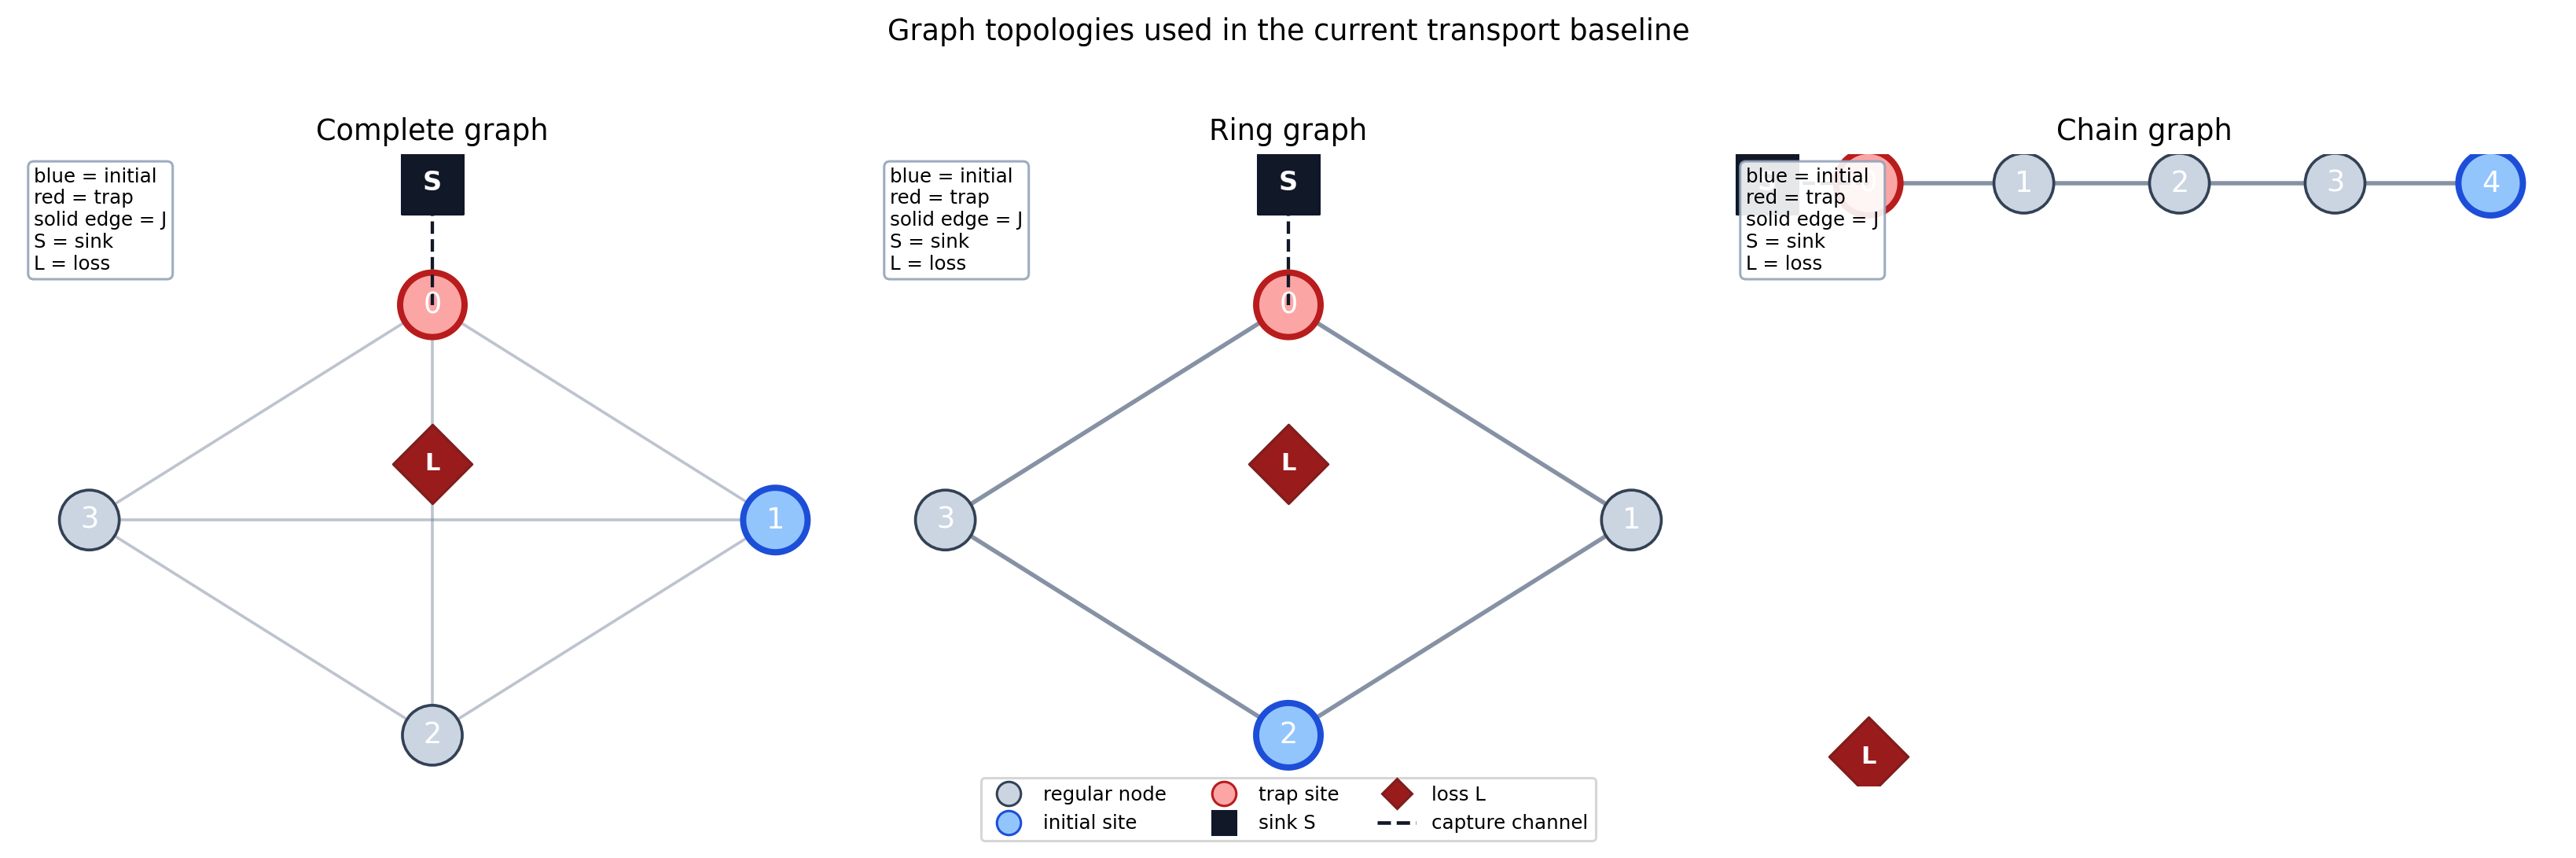
\includegraphics[width=0.95\textwidth]{../../outputs/transport_networks/graph_lab/latest/figures/graph_topology_overview.png}
  \caption{Current baseline topologies. The blue node is the initial site, the red node is the trap site, the square $S$ is the sink, and the square $L$ is the loss channel.}
\end{figure}

\section{Basis states: what does ``the excitation is on node $i$'' mean?}

If the system has $N$ graph nodes, we use the basis
\begin{equation}
\{ \ket{0}, \ket{1}, \ket{2}, \dots, \ket{N-1} \}.
\end{equation}

The interpretation is direct:
\begin{equation}
\ket{i} = \text{``the excitation is localized on node } i \text{''}.
\end{equation}

For a two-site system,
\begin{equation}
\ket{0} = \begin{pmatrix} 1 \\ 0 \end{pmatrix},
\qquad
\ket{1} = \begin{pmatrix} 0 \\ 1 \end{pmatrix}.
\end{equation}

\section{Step 1: the simplest coherent walk}

We begin with the simplest possible case: two nodes, no sink, no loss, and no
dephasing.

\subsection{Two-site Hamiltonian}

If the two sites are coupled with strength $J$, the Hamiltonian is
\begin{equation}
H = J(\ket{0}\bra{1} + \ket{1}\bra{0})
=
\begin{pmatrix}
0 & J \\
J & 0
\end{pmatrix}.
\end{equation}

\subsection{Opening the unitary-evolution calculation}

The unitary evolution operator is
\begin{equation}
U(t)=e^{-iHt}.
\end{equation}

Since
\begin{equation}
H^2 =
\begin{pmatrix}
0 & J \\
J & 0
\end{pmatrix}^2
= J^2 \mathbb{I},
\end{equation}
the exponential series can be summed:
\begin{align}
U(t)
&= \mathbb{I} - iHt - \frac{H^2t^2}{2!} + \frac{iH^3t^3}{3!} + \dots \\
&= \cos(Jt)\,\mathbb{I} - i\sin(Jt)\,\frac{H}{J}.
\end{align}

If the initial state is $\ket{\psi(0)} = \ket{1}$, then
\begin{align}
\ket{\psi(t)}
&= U(t)\ket{1} \\
&= \cos(Jt)\ket{1} - i\sin(Jt)\ket{0}.
\end{align}

Therefore the node populations are
\begin{equation}
P_0(t) = \sin^2(Jt),
\qquad
P_1(t) = \cos^2(Jt).
\end{equation}

This is the simplest coherent walk: the excitation oscillates between the two sites.

\begin{figure}[t]
  \centering
  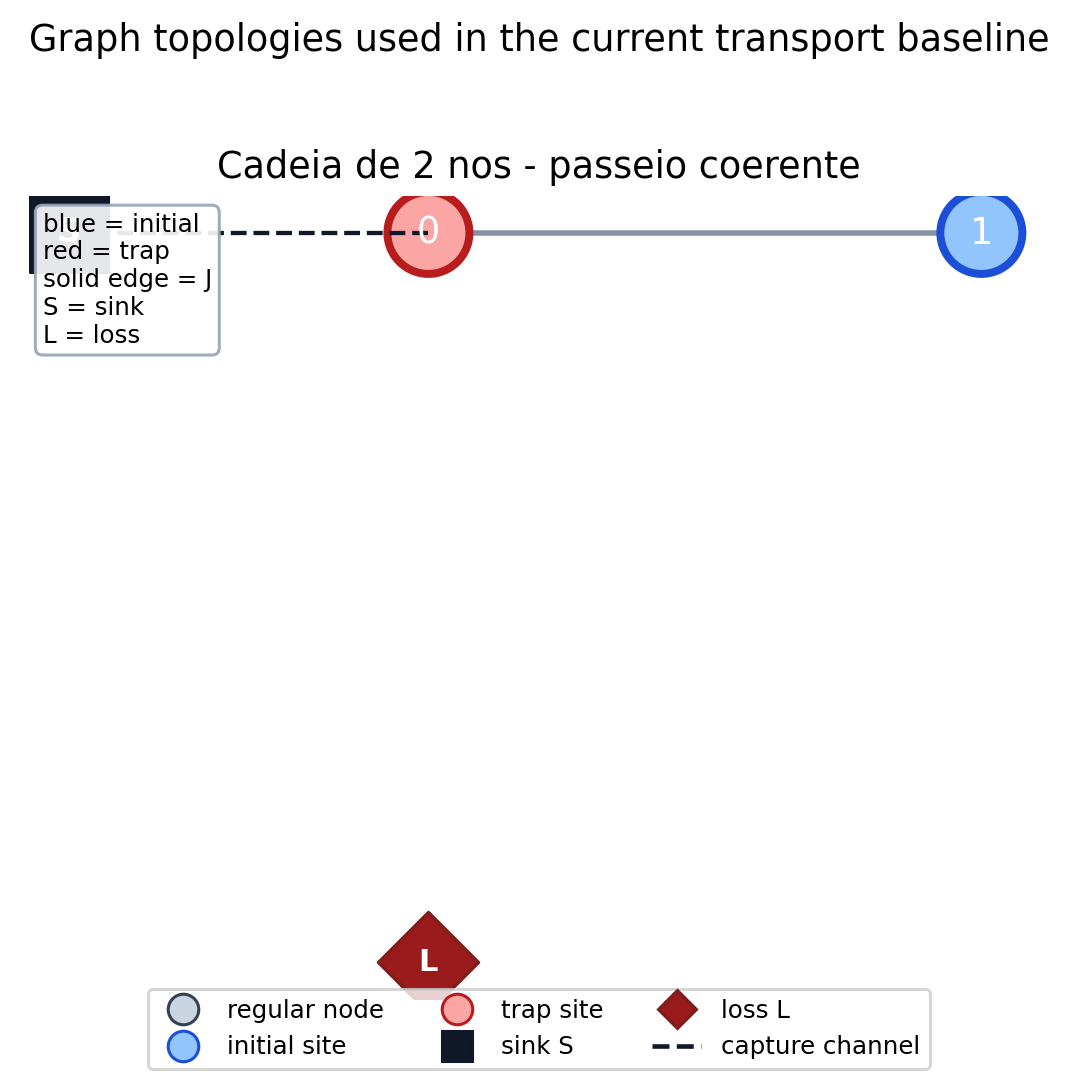
\includegraphics[width=0.55\textwidth]{../../outputs/transport_networks/learning_step1_walk/latest/figures/graph_topology_overview.png}
  \caption{Learning step 1: a two-site chain without sink, loss, or dephasing. The purpose is simply to see the clean coherent oscillation.}
\end{figure}

\section{Why do we move from state vectors to density matrices?}

Once the environment can destroy coherence or remove population, the natural
object becomes the density matrix:
\begin{equation}
\rho = \ket{\psi}\bra{\psi}
\end{equation}
for pure states, and more generally a statistical mixture for mixed states.

For two sites,
\begin{equation}
\rho =
\begin{pmatrix}
\rho_{00} & \rho_{01} \\
\rho_{10} & \rho_{11}
\end{pmatrix}.
\end{equation}

Interpretation:
\begin{itemize}
  \item $\rho_{00}$ and $\rho_{11}$ are populations;
  \item $\rho_{01}$ and $\rho_{10}$ are coherences.
\end{itemize}

\section{From the Schr\"odinger equation to the von Neumann equation}

If the system is closed, the state vector obeys
\begin{equation}
i\frac{d}{dt}\ket{\psi} = H\ket{\psi}.
\end{equation}

Starting from $\rho = \ket{\psi}\bra{\psi}$, we derive
\begin{align}
\frac{d\rho}{dt}
&= \frac{d}{dt}\left(\ket{\psi}\bra{\psi}\right) \\
&= \left(\frac{d\ket{\psi}}{dt}\right)\bra{\psi} + \ket{\psi}\left(\frac{d\bra{\psi}}{dt}\right) \\
&= -iH\rho + i\rho H \\
&= -i[H,\rho].
\end{align}

\section{Opening the commutator explicitly}

Take
\begin{equation}
H =
\begin{pmatrix}
0 & J \\
J & 0
\end{pmatrix},
\qquad
\rho =
\begin{pmatrix}
\rho_{00} & \rho_{01} \\
\rho_{10} & \rho_{11}
\end{pmatrix}.
\end{equation}

Then
\begin{equation}
[H,\rho] =
\begin{pmatrix}
J(\rho_{10}-\rho_{01}) & J(\rho_{11}-\rho_{00}) \\
J(\rho_{00}-\rho_{11}) & J(\rho_{01}-\rho_{10})
\end{pmatrix}.
\end{equation}

Thus
\begin{align}
\dot{\rho}_{00} &= -iJ(\rho_{10}-\rho_{01}), \\
\dot{\rho}_{11} &= -iJ(\rho_{01}-\rho_{10}), \\
\dot{\rho}_{01} &= -iJ(\rho_{11}-\rho_{00}), \\
\dot{\rho}_{10} &= -iJ(\rho_{00}-\rho_{11}).
\end{align}

These equations show explicitly that populations and coherences are coupled.

\section{Open quantum systems and the Lindblad equation}

Now we introduce the main new concept: the system is not perfectly isolated. A
standard effective model for such dynamics is the Lindblad master equation:
\begin{equation}
\frac{d\rho}{dt}
= -i[H,\rho]
+ \sum_k \left(L_k\rho L_k^\dagger - \frac12\{L_k^\dagger L_k,\rho\}\right).
\end{equation}

Interpretation:
\begin{itemize}
  \item $-i[H,\rho]$ is the coherent part;
  \item $L_k$ are dissipative channels;
  \item each $L_k$ represents one effective physical process.
\end{itemize}

This is the standard effective starting point for open quantum systems
\citep{breuer_petruccione_2007, rivas_huelga_2012}.

\section{Dephasing: the first dissipative channel to understand}

In the current laboratory, the most important dissipative channel is dephasing.
On node $i$, it is written as
\begin{equation}
L_i^{(\phi)} = \sqrt{\gamma_{\phi,i}}\,\ket{i}\bra{i}.
\end{equation}

For a two-site system with the same dephasing rate $\gamma_\phi$ on each site,
the dissipative contribution yields
\begin{equation}
\dot{\rho}_{01}\Big|_{\phi} = -\gamma_\phi\,\rho_{01},
\qquad
\dot{\rho}_{10}\Big|_{\phi} = -\gamma_\phi\,\rho_{10}.
\end{equation}

So dephasing mainly kills coherence. That is why a modest amount can suppress
harmful interference, while too much dephasing can suppress transport itself.

\section{What is the sink?}

The \emph{sink} is a success channel. It is not an ordinary graph node. It represents
\begin{quote}
``the excitation has arrived at the useful target''.
\end{quote}

If the trap site is $\ket{t}$, then we write
\begin{equation}
L^{(\mathrm{sink})} = \sqrt{\kappa}\,\ket{s}\bra{t},
\end{equation}
where $\ket{s}$ is the sink state.

The main laboratory observable is
\begin{equation}
\eta(T)=\rho_{ss}(T).
\end{equation}

The sink population therefore measures success, not generic motion through the graph.

\section{What is loss?}

The \emph{loss} channel is another absorbing state, but it represents failure:
\begin{equation}
L_i^{(\mathrm{loss})} = \sqrt{\Gamma_i}\,\ket{\ell}\bra{i}.
\end{equation}

Population leaving the graph can therefore have two destinations:
\begin{itemize}
  \item \textbf{sink}: successful capture;
  \item \textbf{loss}: parasitic dissipation.
\end{itemize}

\section{Laboratory observables}

The three main observables are:
\begin{enumerate}
  \item \textbf{sink efficiency}
  \begin{equation}
  \eta(T)=\rho_{ss}(T);
  \end{equation}
  \item \textbf{population dynamics}
  \begin{equation}
  P_i(t)=\rho_{ii}(t);
  \end{equation}
  \item \textbf{coherence}
  \begin{equation}
  C_{\ell_1}(\rho)=\sum_{i\neq j}|\rho_{ij}|.
  \end{equation}
\end{enumerate}

\section{Three simple learning simulations}

\subsection{Step 1: coherent walk}

Configuration file:
\begin{quote}
\texttt{configs/transport\_learning\_step1\_walk.json}
\end{quote}

Here the sink and loss are absent, so $\eta(T)=0$ by construction. The point is
simply to see coherent oscillation.

\begin{figure}[t]
  \centering
  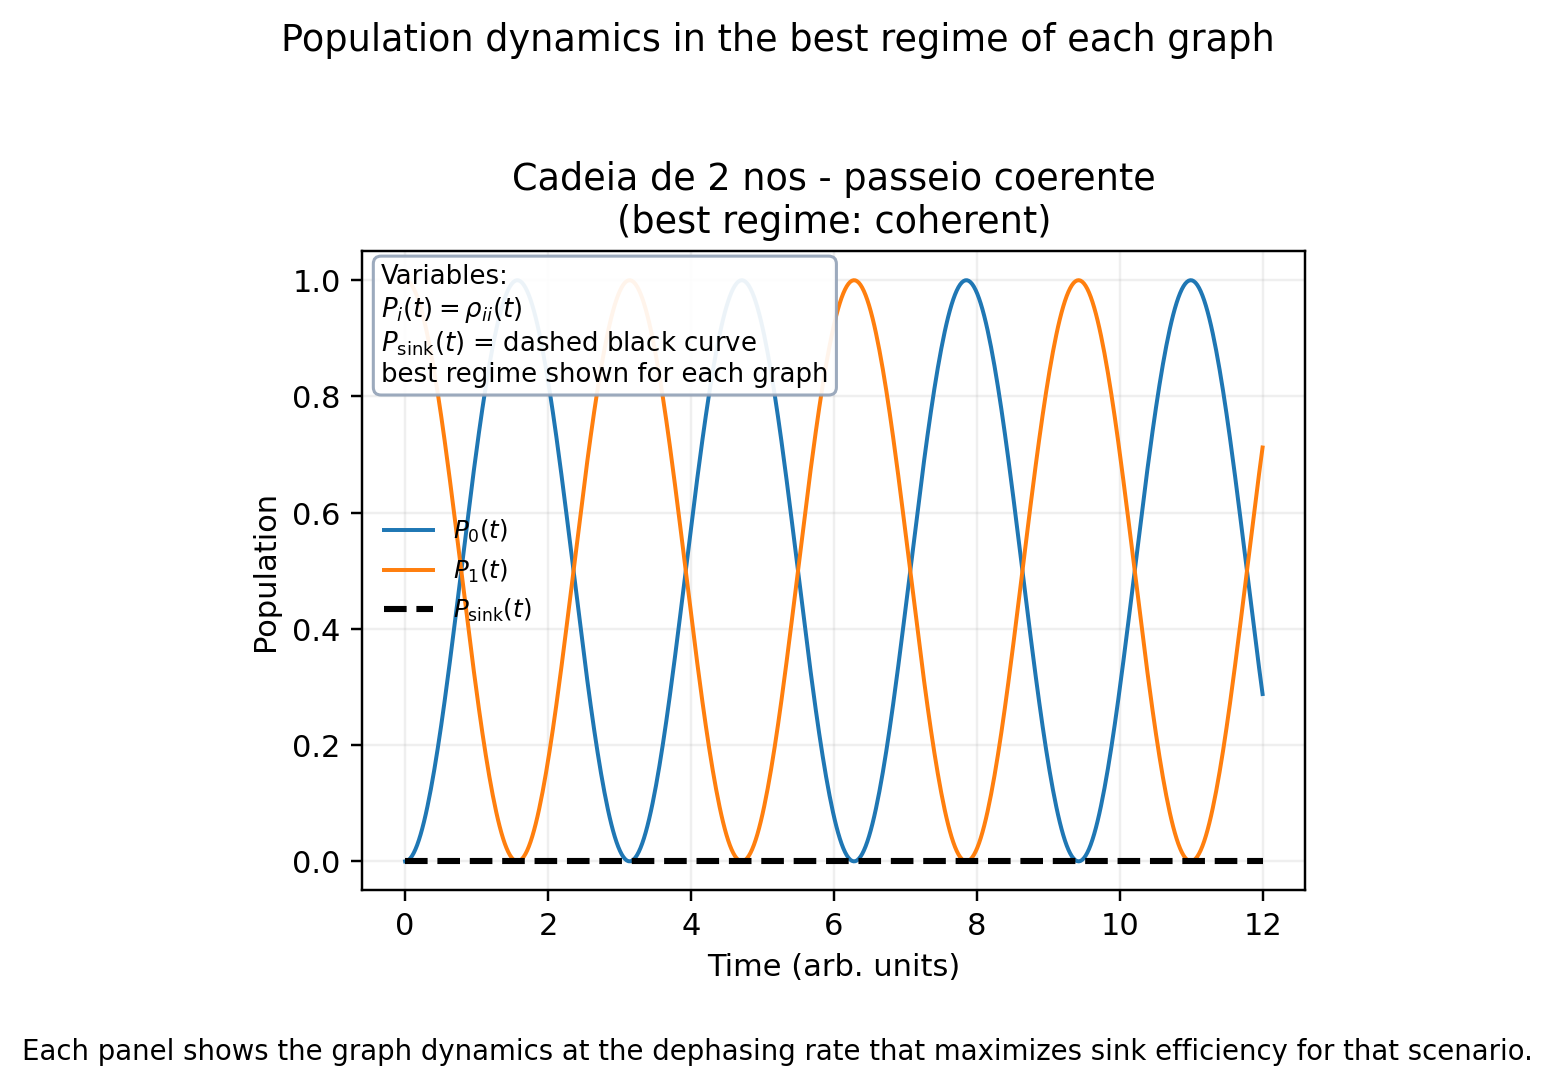
\includegraphics[width=0.60\textwidth]{../../outputs/transport_networks/learning_step1_walk/latest/figures/population_dynamics_by_graph.png}
  \caption{Step 1: population dynamics for a two-site system without dissipation or sink.}
\end{figure}

\subsection{Step 2: introducing the sink}

Configuration file:
\begin{quote}
\texttt{configs/transport\_learning\_step2\_sink.json}
\end{quote}

Now the excitation moves through a three-site chain and can be captured once it reaches the trap site.

\begin{figure}[t]
  \centering
  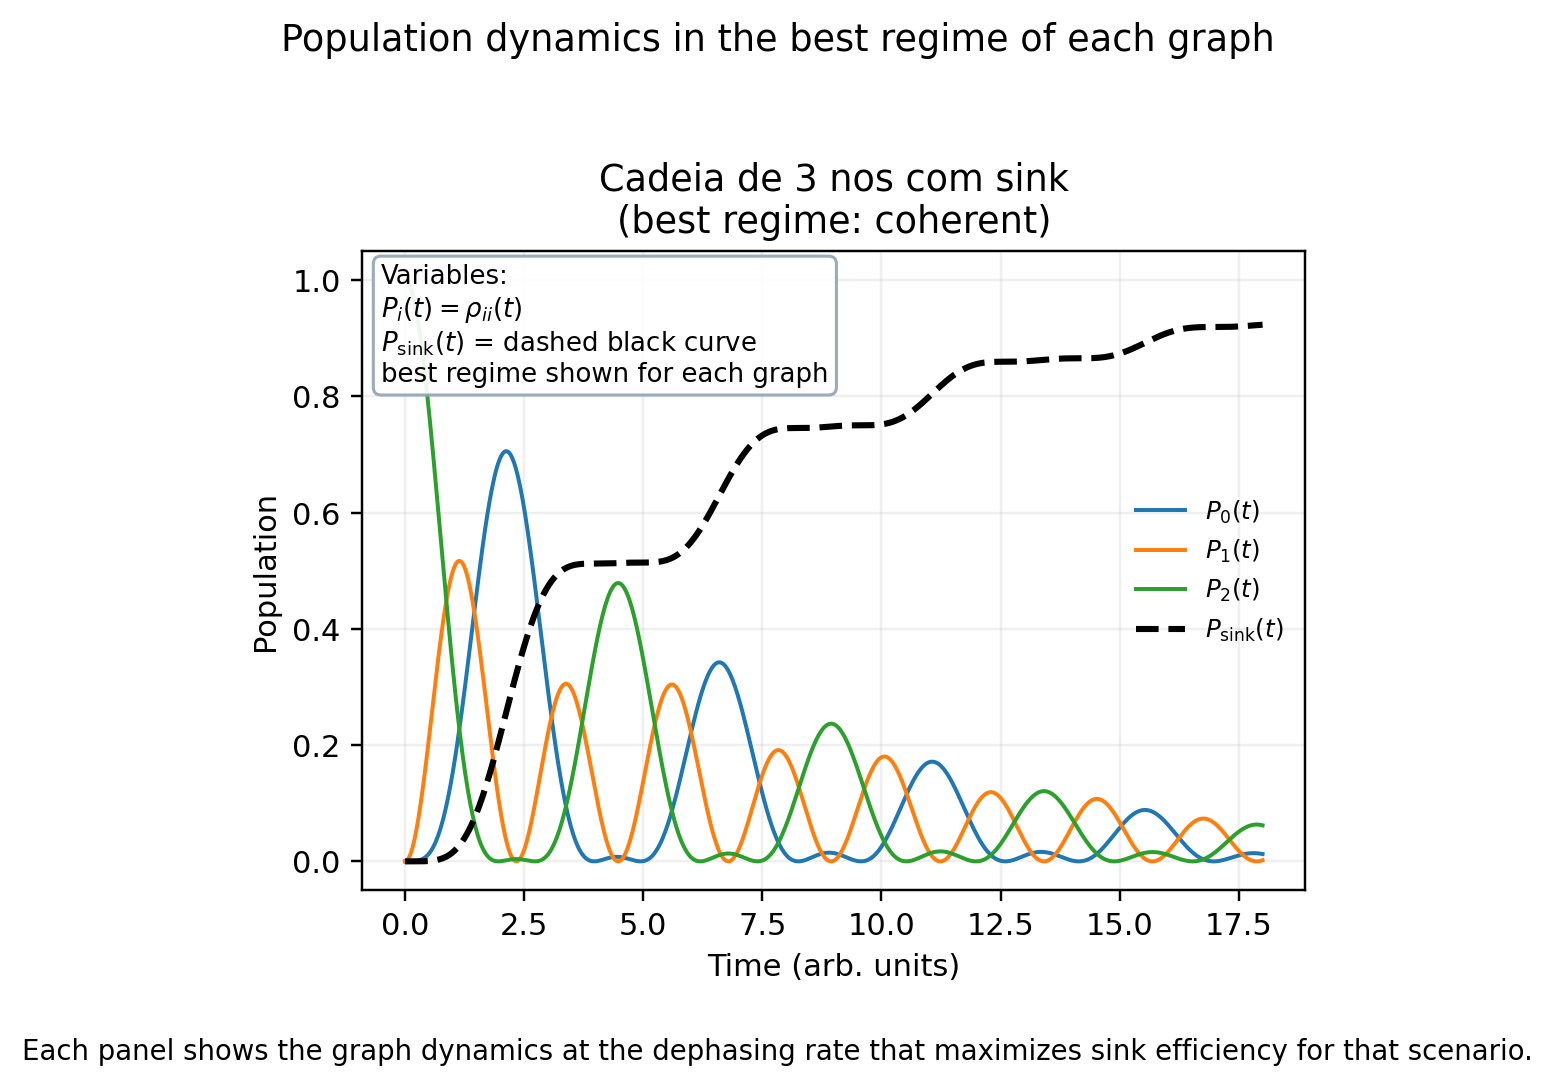
\includegraphics[width=0.60\textwidth]{../../outputs/transport_networks/learning_step2_sink/latest/figures/population_dynamics_by_graph.png}
  \caption{Step 2: with an active sink, the sink population grows in time. This is the first figure that should be read as successful transport.}
\end{figure}

\subsection{Step 3: introducing dephasing}

Configuration file:
\begin{quote}
\texttt{configs/transport\_learning\_step3\_dephasing.json}
\end{quote}

Now the genuinely interesting question appears: can a small amount of dephasing improve transport? In the current example, yes. The maximum efficiency does not occur at $\gamma_\phi=0$, but at an intermediate value.

\begin{figure}[t]
  \centering
  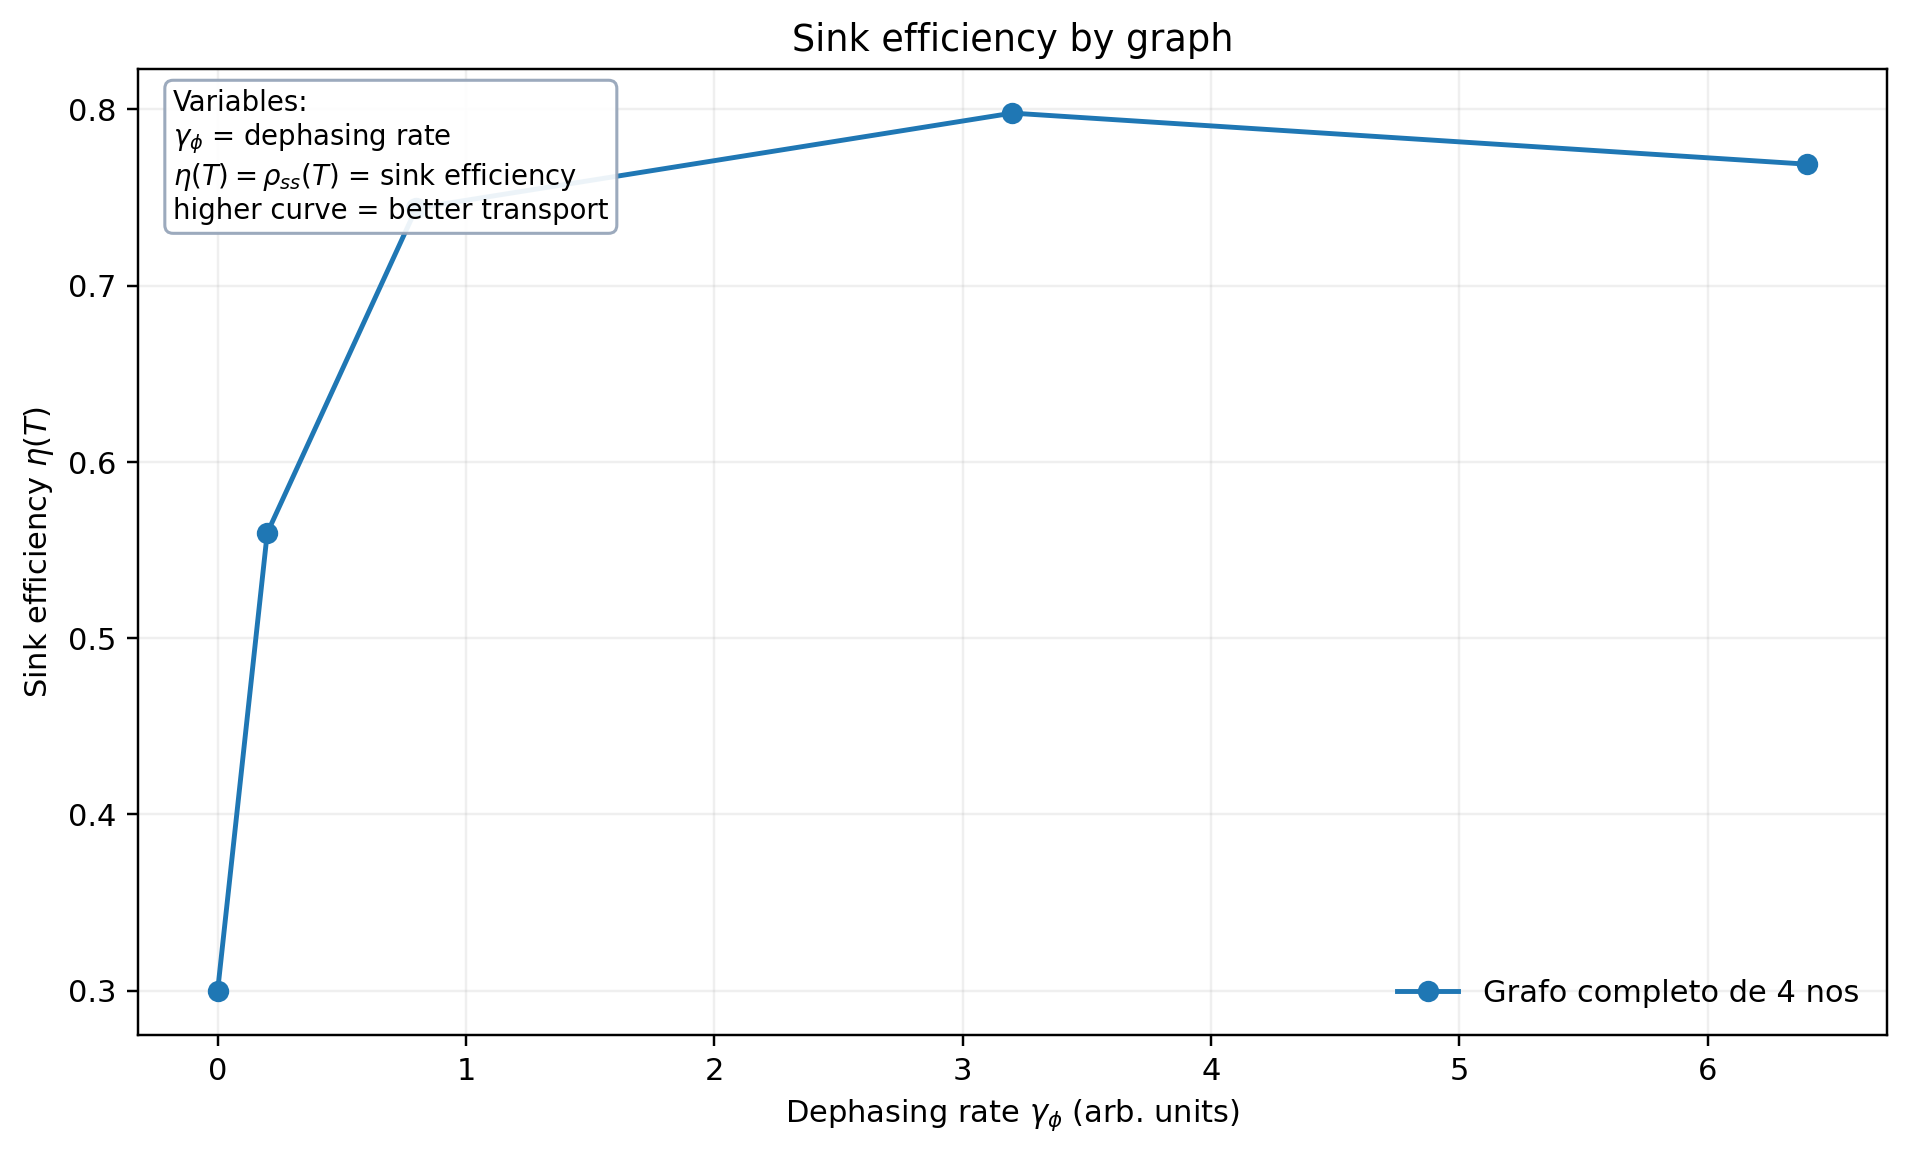
\includegraphics[width=0.88\textwidth]{../../outputs/transport_networks/learning_step3_dephasing/latest/figures/sink_efficiency_by_graph.png}
  \caption{Step 3: an example in which the transport efficiency improves when dephasing increases from zero to an intermediate regime.}
\end{figure}

\section{What has already been simulated}

The current laboratory already contains three pedagogical simulations and one larger baseline comparison.

\begin{table}[t]
\centering
\caption{Learning-path results generated directly from the current simulation artifacts.}
\begin{tabular}{llcccc}
\toprule
Step & Scenario & Best regime & $\eta_{\mathrm{coh}}$ & $\eta_{\mathrm{best}}$ & $\gamma_{\phi}^{\mathrm{best}}$ \\
\midrule
Step 1 & Two-site coherent walk & coherent & 0.000 & 0.000 & 0.000 \\
Step 2 & Three-site chain with sink & coherent & 0.923 & 0.923 & 0.000 \\
Step 3 & Four-site complete graph with dephasing scan & intermediate & 0.300 & 0.798 & 3.200 \\
\bottomrule
\end{tabular}
\end{table}


The present learning-path data say the following:
\begin{itemize}
  \item \textbf{Step 1}: the two-site walk is purely coherent, so the sink efficiency is zero by construction.
  \item \textbf{Step 2}: once the sink is introduced, the three-site chain reaches $\eta \approx 0.923$, so most of the excitation ends in the useful target.
  \item \textbf{Step 3}: on the four-site complete graph, the coherent regime is poor ($\eta \approx 0.300$), but an intermediate dephasing rate improves the efficiency to $\eta \approx 0.798$.
\end{itemize}

\begin{table}[t]
\centering
\caption{Baseline graph-comparison results generated from the current laboratory run.}
\begin{tabular}{lcccc}
\toprule
Scenario & Best regime & $\eta_{\mathrm{coh}}$ & $\eta_{\mathrm{best}}$ & $\gamma_{\phi}^{\mathrm{best}}$ \\
\midrule
Complete graph & intermediate & 0.300 & 0.798 & 3.200 \\
Ring graph & coherent & 0.795 & 0.795 & 0.000 \\
Chain graph & coherent & 0.812 & 0.812 & 0.000 \\
\bottomrule
\end{tabular}
\end{table}


For the larger baseline comparison:
\begin{itemize}
  \item \textbf{Complete graph}: best regime is intermediate, with a strong dephasing-assisted gain.
  \item \textbf{Ring graph}: best regime is coherent for the current parameter set.
  \item \textbf{Chain graph}: best regime is also coherent, and large dephasing is strongly harmful.
\end{itemize}

\begin{figure}[t]
  \centering
  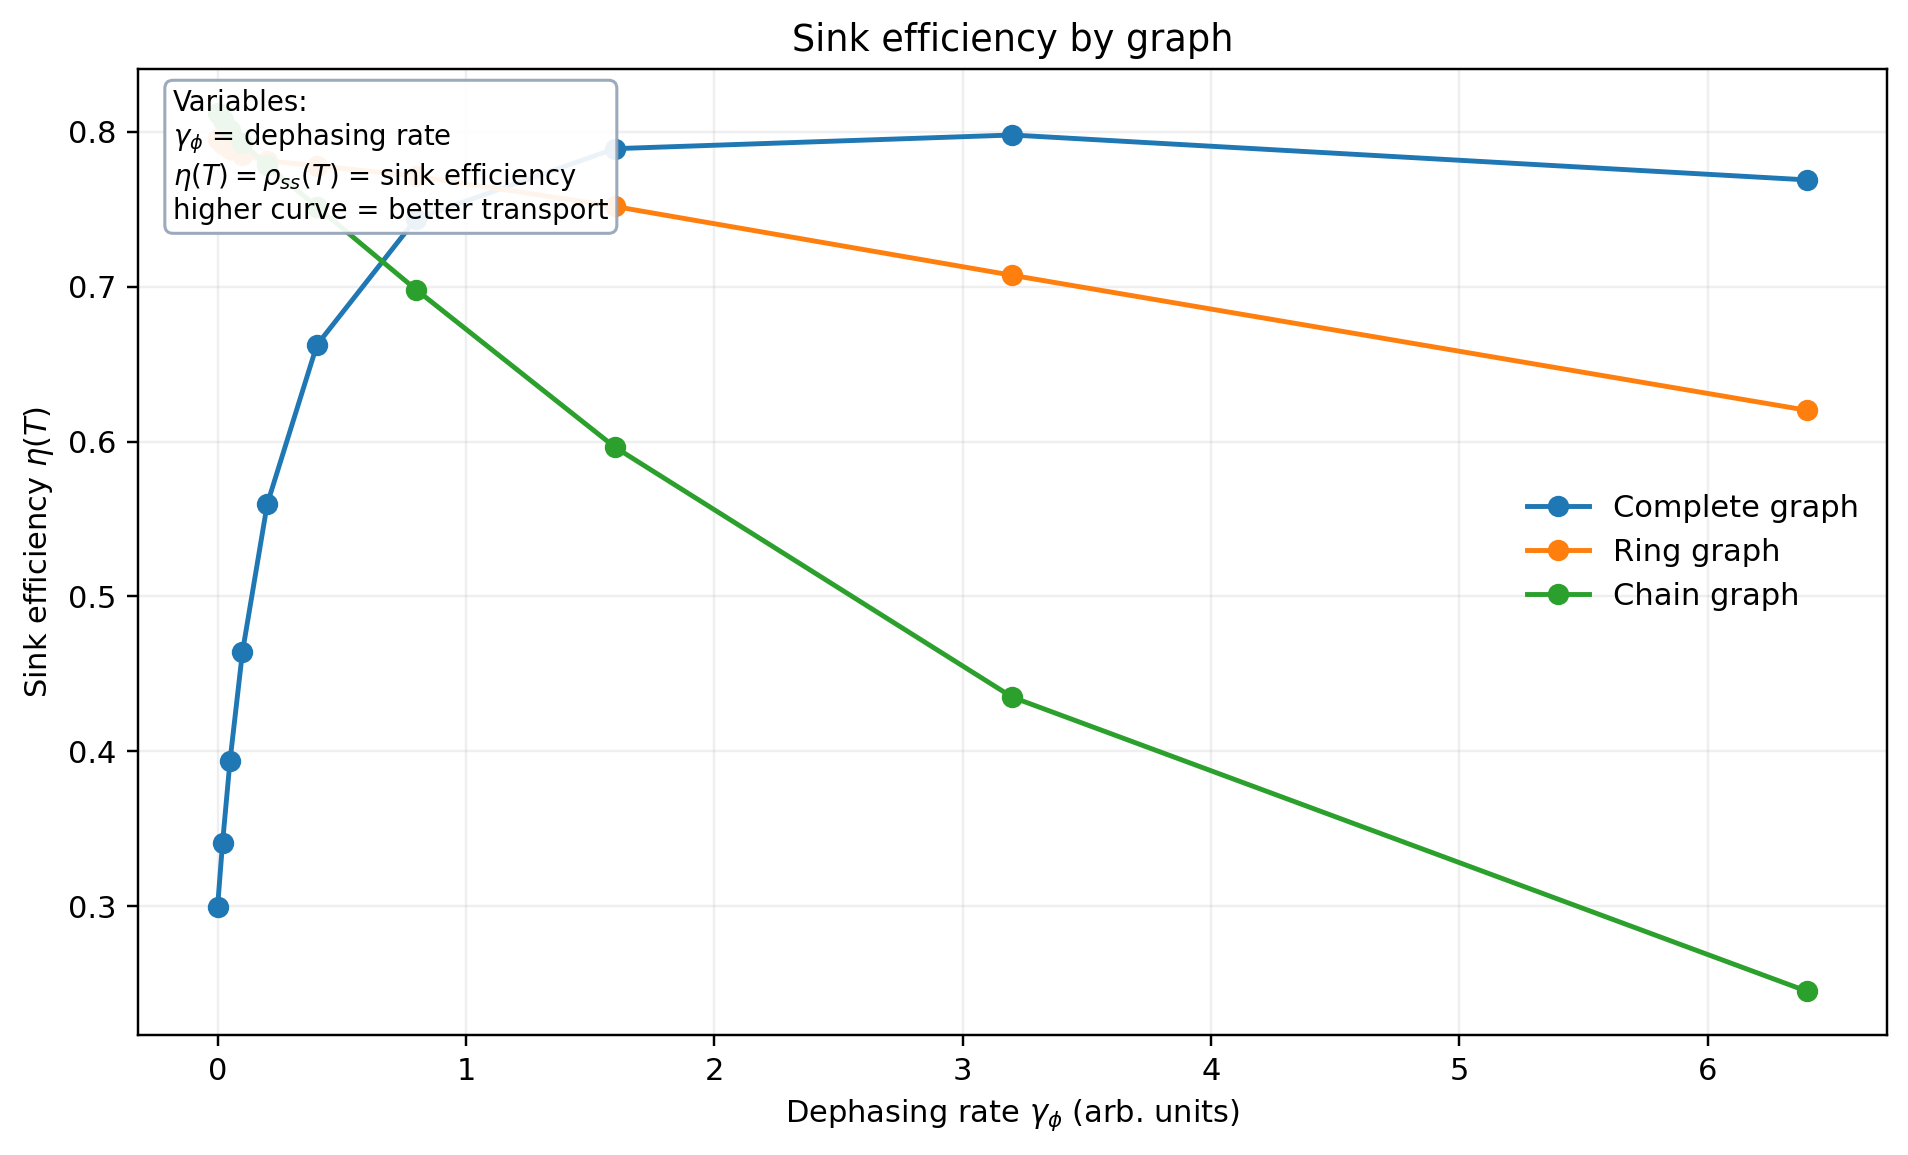
\includegraphics[width=0.90\textwidth]{../../outputs/transport_networks/graph_lab/latest/figures/sink_efficiency_by_graph.png}
  \caption{Main baseline comparison between graph topologies. The complete graph exhibits an optimal intermediate regime, whereas the chain and ring are best in the coherent limit for the current parameters.}
\end{figure}

\begin{figure}[t]
  \centering
  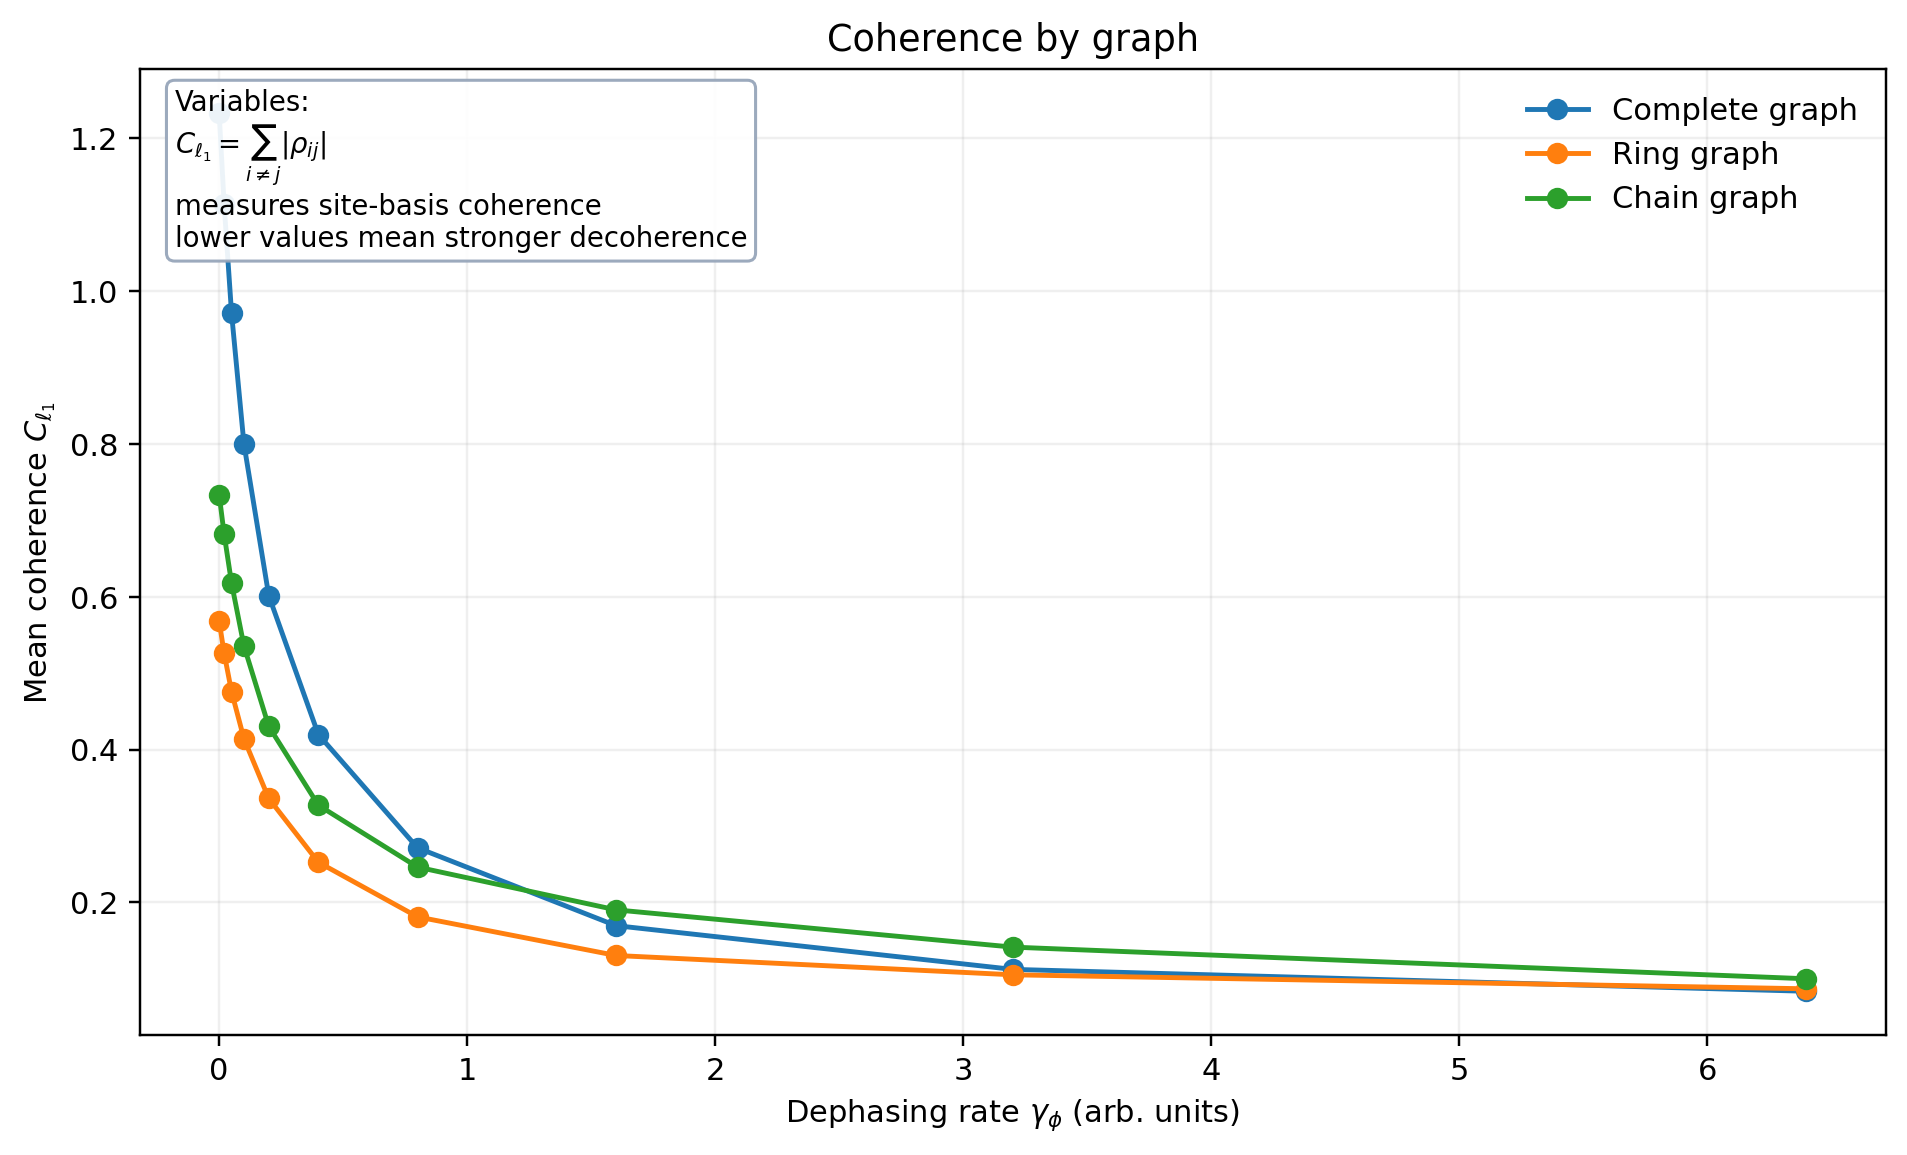
\includegraphics[width=0.90\textwidth]{../../outputs/transport_networks/graph_lab/latest/figures/coherence_by_graph.png}
  \caption{Baseline coherence comparison. The chain preserves the largest coherence in the optimal regime, while the complete graph reaches its best transport efficiency with substantially lower coherence.}
\end{figure}

\section{Short solved exercises}

\subsection*{Exercise 1: two-site coherent walk}

\textbf{Problem.} Consider
\begin{equation}
H = J(\ket{0}\bra{1}+\ket{1}\bra{0})
\end{equation}
and the initial state $\ket{\psi(0)}=\ket{1}$. Find $P_0(t)$.

\textbf{Solution.} From the derivation above,
\begin{equation}
\ket{\psi(t)}=\cos(Jt)\ket{1}-i\sin(Jt)\ket{0},
\end{equation}
so
\begin{equation}
P_0(t)=|\bra{0}\psi(t)\rangle|^2=\sin^2(Jt).
\end{equation}

\subsection*{Exercise 2: sink versus loss}

\textbf{Problem.} At the final time $T$, suppose the state has $\rho_{ss}(T)=0.80$ and $\rho_{\ell\ell}(T)=0.15$. What do these numbers mean?

\textbf{Solution.} The sink population is the transport efficiency:
\begin{equation}
\eta(T)=\rho_{ss}(T)=0.80.
\end{equation}
So $80\%$ of the excitation ended in the useful target. The loss population says that $15\%$ of the excitation was removed by parasitic dissipation. The remaining population is still distributed among graph nodes.

\subsection*{Exercise 3: identifying the best regime}

\textbf{Problem.} A graph has $\eta_{\mathrm{coh}}=0.30$, $\eta_{\mathrm{best}}=0.80$, and $\gamma_{\phi}^{\mathrm{best}}=3.2$. Which regime is preferred?

\textbf{Solution.} Since the best efficiency is much larger than the coherent one and it occurs at a nonzero dephasing rate, the preferred regime is \textbf{intermediate dephasing}. This is exactly what the current complete-graph simulation shows.

\subsection*{Exercise 4: reading a coherence plot}

\textbf{Problem.} If the coherence decreases strongly while the sink efficiency increases, is that automatically a contradiction?

\textbf{Solution.} No. In these transport problems, some coherence is useful, but excessive coherent interference can also trap the excitation in unfavorable pathways. A modest reduction in coherence can therefore improve transport if it suppresses destructive interference without freezing the dynamics.

\section{How to use the laboratory without getting lost}

The most efficient workflow is:
\begin{enumerate}
  \item run step 1 and understand coherent oscillation only;
  \item run step 2 and understand what the sink actually measures;
  \item run step 3 and understand what dephasing changes;
  \item only then move to the full baseline comparison.
\end{enumerate}

The most important files are:
\begin{itemize}
  \item \texttt{configs/transport\_learning\_step1\_walk.json};
  \item \texttt{configs/transport\_learning\_step2\_sink.json};
  \item \texttt{configs/transport\_learning\_step3\_dephasing.json};
  \item \texttt{configs/transport\_graph\_lab\_config.json};
  \item \texttt{scripts/run\_transport\_learning\_path.py};
  \item \texttt{scripts/run\_transport\_graph\_lab.py}.
\end{itemize}

\section{Closing remarks}

If you keep only one idea from this tutorial, let it be this:
\begin{quote}
The laboratory is not simulating an arbitrary random walk on a graph. It is simulating how a quantum excitation moves, loses coherence, gets removed by parasitic channels, or reaches the useful target.
\end{quote}

In other words:
\begin{itemize}
  \item the nodes say where the excitation can be;
  \item the Hamiltonian says how it moves;
  \item Lindblad terms say how the environment acts;
  \item the sink measures success;
  \item the loss channel measures failure;
  \item the topology changes all of that.
\end{itemize}

\bibliographystyle{unsrtnat}
\bibliography{references}

\end{document}
